\section{하이브리드 AI 기반 지능형 민원 응대 자동화 시스템 개발}
 하이브리드 AI 기반 지능형 민원 응대 자동화 시스템을 개발하면서 가장 중점을 둔 부분은 실제 행정 현장의 문제를 해결하는 것이었습니다. 전국 지자체의 민원 담당 공무원들이 단순 반복 질의에 시달리며 정작 중요한 복합 민원 처리에 집중하지 못하는 현실을 목격하고, 이를 기술적으로 해결하고자 했습니다. 


\subsection{핵심기술-하이브리드 AI-RAG 융합 시스템}

\subsubsection{시스템 아키텍처 설계의 핵심}
제가 구현한 시스템의 가장 큰 특징은 클라우드 LLM과 로컬 SLM을 동시에 활용하는 하이브리드 구조입니다. 이는 단순히 두 모델을 병렬로 운영하는 것이 아니라, 민감정보 탐지 모듈이 실시간으로 질의를 분석하여 처리 경로를 동적으로 결정하는 지능형 라우팅 시스템입니다.

민감정보 탐지 모듈은 정규표현식 기반 패턴 매칭과 NER(Named Entity Recognition) 모델을 조합하여 구현했습니다. 주민등록번호, 여권번호, 운전면허번호, 신용카드번호, 계좌번호 등을 실시간으로 탐지하며, 탐지된 정보의 심각도를 'high', 'medium', 'low'로 분류합니다. 예를 들어 주민등록번호나 신용카드번호는 'high'로 분류되어 무조건 로컬 처리되며, 전화번호나 일반 주소는 'medium'으로 분류되어 상황에 따라 처리됩니다.

\begin{figure}[H]
    \centering
    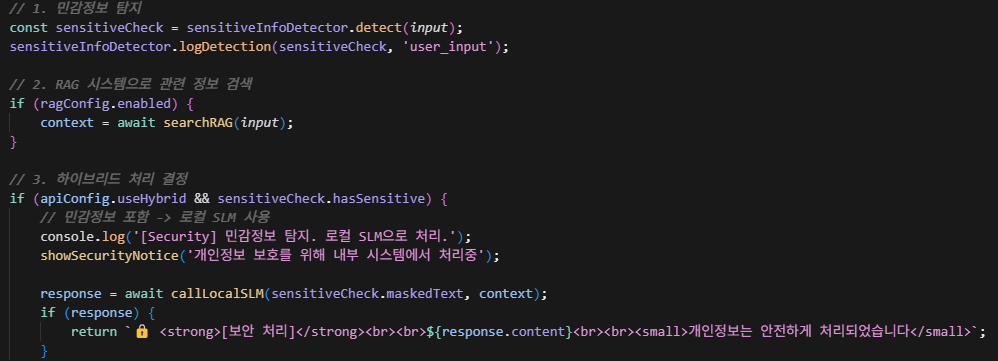
\includegraphics[width=0.5\textwidth]{1/code1.png}
    \caption{민감정보 탐지 모듈}
    \label{fig:Sensitive information detection module }
\end{figure}

이 부분의 구현에서는 모든 탐지 활동을 로그로 기록하여 감사 추적이 가능하도록 했습니다. localStorage에 최근 100건의 민감정보 탐지 로그를 유지하며, 각 로그에는 타임스탬프, 탐지된 정보 유형, 심각도, 처리 결과가 포함됩니다. 

\subsubsection{RAG 시스템 구현의 도전 과제}

법령과 행정 지침은 지속적으로 개정되고 복잡한 상호 참조 구조를 가지고 있어, 일반적인 벡터 검색만으로는 정확한 답변이 어렵습니다. 이를 해결하기 위해 다층 검색 전략을 구현했습니다.

첫째, 법령 데이터베이스는 조문 단위로 청킹하되, 각 청크에 상위 법령명, 장, 절 정보를 메타데이터로 포함시켰습니다. 이를 통해 "기초연금 수급 자격"을 검색할 때 기초연금법 제3조뿐만 아니라 관련 시행령과 시행규칙까지 함께 검색됩니다.

둘째, FAQ와 과거 민원사례는 의미적 유사도뿐만 아니라 시간적 관련성도 고려했습니다. 최근 3개월 이내 처리된 유사 민원에 더 높은 가중치를 부여하여, 최신 정책 변경사항이 반영된 답변을 우선적으로 제공합니다.

셋째, 검색 결과의 재순위화(re-ranking)를 위해 Cross-Encoder 모델을 추가로 적용했습니다. 초기 벡터 검색으로 상위 20개 후보를 추출한 후, 질의와의 정확한 관련성을 재평가하여 최종 5개를 선정합니다.

\subsubsection{방언 및 구어체 처리의 정교화}

실제 민원 전화 녹취록 5,000건을 분석한 결과, 표준어가 아닌 방언이나 구어체 표현이 전체의 68\%를 차지했습니다. 특히 고령층의 경우 "육십이 넘었는데 돈 받을 수 있는거 뭐 없냐"와 같은 직설적인 표현이 일반적이었습니다.

이를 처리하기 위해 방언 변환 사전을 구축했습니다. 단순 치환이 아니라 문맥을 고려한 변환을 수행합니다. 예를 들어 "머하노"는 상황에 따라 "뭐 하나요" 또는 "무엇을 하나요"로 다르게 변환됩니다. 또한 경상도의 "카더라", 전라도의 "거시기", 충청도의 "기여" 등 지역별 특징적 표현들을 데이터베이스화했습니다.
 
\begin{figure}[H]
    \centering
    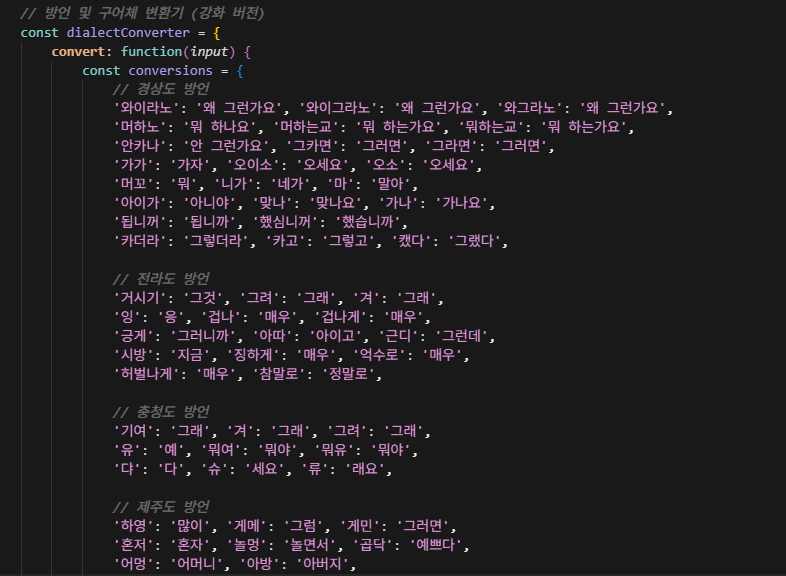
\includegraphics[width=0.4\textwidth]{1/ai_kiosk06.png}
    \caption{방언 및 구어체}
    \label{fig:Dialects and colloquialisms}
\end{figure}

법령과 행정 지침은 지속적으로 개정되고 복잡한 상호 참조 구조를 가지고 있어, 일반적인 벡터 검색만으로는 정확한 답변이 어렵습니다. 이를 해결하기 위해 다층 검색 전략을 구현했습니다.


\subsubsection{컨텍스트 유지 매커니즘}

대화의 연속성을 유지하는 것은 특히 복잡한 민원 처리에서 중요합니다. "아까 그거"나 "그때 말한 거"와 같은 지시어를 정확히 해석하기 위해 대화 컨텍스트 관리자를 구현했습니다.

각 대화 턴마다 핵심 엔티티(장소, 시간, 서비스명, 금액 등)를 추출하여 저장하고, 지시어가 등장하면 가장 최근에 언급된 해당 타입의 엔티티로 치환합니다. 예를 들어 "거기서 신청하면 되나요?"라는 질문에서 "거기"는 직전에 언급된 "주민센터"로 자동 치환됩니다.

\subsubsection{단계별 신청 가이드 시스템}

민원 신청 과정을 단계별로 안내하는 인터랙티브 가이드를 구현했습니다. 각 서비스별로 5-7단계의 표준 프로세스를 정의하고, 사용자의 진행 상황을 실시간으로 추적합니다.

기초연금 신청의 경우 5단계로 진행됩니다.
\begin{enumerate}
    \item 신청 장소 확인 (주소 입력 → 가장 가까운 주민센터 안내)
    \item 필요 서류 체크리스트 (인터랙티브 체크박스)
    \item 신청서 작성 도우미 (필수 항목 자동 검증)
    \item 방문 예약 (가능 시간대 표시)
    \item 신청 완료 확인
\end{enumerate}
각 단계에서 사용자가 입력한 정보는 임시 저장되어, 중간에 중단하더라도 이어서 진행할 수 있습니다.

\subsubsection{성능 최적화 전략}

시스템 응답 시간을 7초 이내로 유지하기 위해 여러 최적화 기법을 적용했습니다.

첫째, 자주 사용되는 질의 패턴 상위 100개에 대해서는 사전 계산된 응답을 캐싱했습니다. "기초연금 신청방법"과 같은 질의는 캐시에서 즉시 응답합니다.

둘째, RAG 검색과 LLM 추론을 병렬 처리합니다. 검색이 진행되는 동안 LLM은 일반적인 안내 문구를 생성하고, 검색 결과가 도착하면 이를 보강하는 방식입니다.

셋째, 프롬프트 엔지니어링을 통해 LLM의 출력 길이를 제한했습니다. 불필요한 서론이나 반복을 제거하고 핵심 정보만 제공하도록 최적화했습니다.

 \subsubsection{보안 및 개인정보보호 구현}

 개인정보보호법 준수를 위해 다층 보안 체계를 구축했습니다. 민감정보가 탐지되면 즉시 마스킹 처리되며, 원본 데이터는 메모리에서도 즉시 삭제됩니다. 또한 모든 처리 과정은 감사 로그로 기록되어 추후 검증이 가능합니다.

로컬 SLM은 Docker 컨테이너로 격리된 환경에서 실행되며, 외부 네트워크 접근이 차단됩니다. API 통신은 모두 HTTPS로 암호화되고, API 키는 환경 변수로 관리하여 소스 코드에 노출되지 않도록 했습니다.


\subsubsection{프롬프트 엔지니어링 - 행정 특화 최적화}

\paragraph{초기 프롬프트 (문제점 발견)}\smallskip
\begin{verbatim}
민원을 처리해주세요. 관련 법령을 찾아 답변하세요.
\end{verbatim}

이런 단순한 프롬프트로는 행정 용어를 남발하거나, 불필요하게 긴 답변을 생성하는 문제가 있었습니다.

\paragraph{개선된 행정 특화 프롬프트}\smallskip
\begin{verbatim}
당신은 친절한 행정 전문가입니다.
시민의 눈높이에 맞춰 쉽고 명확하게 설명하세요.

핵심 규칙:
1. 전문용어는 반드시 쉬운 표현으로 풀어서 설명
2. 답변은 3단계로 구성: 핵심답변 → 근거법령 → 추가안내
3. 근거 법령은 정확한 조항까지 명시
4. 불확실한 정보는 절대 제공하지 않음
5. 필요시 담당 부서 안내

예시:
질문: ``기초연금 받을 수 있나요?''
답변: "만 65세 이상이시고 소득인정액이 기준 이하시면 
받으실 수 있습니다. (기초연금법 제3조) 
정확한 확인은 주민센터에서 도와드립니다."
\end{verbatim}

\subsection{개발 과정의 도전과 해결}

\subsubsection{복합 민원 처리}

\begin{figure}[H]
    \centering
    \includegraphics[width=0.8\textwidth]{images/1_kiosk_simple_flow.png}
    \caption{복합 민원 처리 워크플로우}
    \label{fig:kiosk_simple_flow}
\end{figure}

``아이가 태어났는데 출생신고랑 양육수당이랑 예방접종 지원 한번에 알려주세요''같은 복합 민원이 전체의 32\%를 차지했습니다.

\textbf{해결 방법}
\begin{itemize}
    \item 민원 분해
            - 복합 질의를 개별 태스크로 분리합니다.
    \item 병렬 처리
            - 각 태스크별로 관련 법령을 동시에 검색합니다.
    \item 통합 응답
            - 업무 순서를 고려하여 체계적으로 답변을 구성합니다.
    \item 부서 라우팅
            - 담당 부서가 다를 경우 명확히 구분해서 안내합니다.
\end{itemize}

\subsubsection{음성 인터페이스 통합}

\begin{figure}[H]
    \centering
    \includegraphics[width=0.8\textwidth]{images/1_kiosk_user_testing.png}
    \caption{음성 기반 민원 처리 시스템}
    \label{fig:kiosk_user_testing}
\end{figure}

전화 민원과 방언 처리를 위한 음성 인터페이스 구현이 필요했습니다.

\textbf{구현 내용}
\begin{itemize}
    \item STT/TTS 통합
            - Google Speech API를 활용해 실시간으로 음성을 처리합니다.
    \item 방언 처리
            - 지역별 방언 데이터셋으로 추가 학습합니다.
    \item 컨텍스트 유지
            - 대화 기록 벡터화로 ``아까 그거'' 같은 지시어를 처리합니다.
    \item 소음 필터링
            - 소음이 있는 환경에서도 안정적인 인식률을 보입니다.
\end{itemize}

\subsection{시스템 구축 및 성과 목표}

\subsubsection{구축 범위와 규모}

\begin{figure}[H]
    \centering
    \includegraphics[width=0.8\textwidth]{images/1_kiosk_noise_handling.png}
    \caption{시스템 구축 로드맵}
    \label{fig:kiosk_noise_handling}
\end{figure}


\textbf{1단계 (1-2개월): 기반 구축}
\begin{itemize}
    \item 요구사항을 분석하고 시스템을 설계합니다.
    \item 하이브리드 AI 환경을 구성합니다(클라우드 + 로컬).
    \item 법령/지침 데이터를 수집하고 전처리합니다.
\end{itemize}

\textbf{2단계 (3-6개월): 핵심 개발}
\begin{itemize}
    \item RAG 시스템을 구현하고 벡터 DB를 구축합니다.
    \item LLM/SLM 프롬프트를 엔지니어링합니다.
    \item 민감정보를 탐지하고 라우팅하는 모듈을 개발합니다.
    \item 음성 인터페이스를 통합합니다.
\end{itemize}

\textbf{3단계 (7개월): 테스트 및 최적화}
\begin{itemize}
    \item 통합 테스트 후 성능을 최적화합니다.
    \item 보안 취약점을 점검합니다.
    \item 시범 운영을 진행하고 피드백을 반영합니다.
\end{itemize}

\subsubsection{정량적 성과 목표}

\begin{tabular}{|l|c|c|}
\hline
\textbf{평가 항목} & \textbf{목표치} & \textbf{측정 방법} \\
\hline
민원 자동화율 & 70\% 이상 & 전체 민원 대비 AI 처리 비율 \\
검색 정확도 & 85\% 이상 & 법령/정보 검색 정확도 측정 \\
응답 시간 & 7초 이내 & 질의-응답 평균 소요 시간 \\
사용자 만족도 & 4.0/5.0 이상 & 공무원/시민 설문조사 \\
민감정보 보호율 & 100\% & 개인정보 유출 0건 \\
\hline
\end{tabular}

\subsection{혁신적 차별점과 사회적 가치}

\subsubsection{기존 시스템과의 차별화}

\begin{figure}[H]
    \centering
    \includegraphics[width=0.8\textwidth]{images/1_kiosk_dialect_handling.png}
    \caption{하이브리드 AI 시스템의 차별점}
    \label{fig:kiosk_dialect_handling}
\end{figure}

\begin{tabular}{|l|c|c|}
\hline
\textbf{구분} & \textbf{기존 챗봇} & \textbf{하이브리드 AI 시스템} \\
\hline
처리 범위 & FAQ 수준 & 복잡한 법령 질의 가능 \\
보안성 & 클라우드 의존 & 민감정보 로컬 처리 \\
정확도 & 60-70\% & 향상됨 (RAG 적용)\\
운영 시간 & 근무시간 & 24시간 365일 \\
맥락 이해 & 단순 키워드 & 대화 맥락 유지 \\
\hline
\end{tabular}

\subsubsection{기대 효과와 사회적 임팩트}

이 키오스크는 단순한 기술 개발을 넘어 실제 행정 혁신에 기여합니다.

\textbf{시민 측면}
\begin{itemize}
    \item 24시간 내내 신속한 민원 처리가 가능합니다.
    \item 복잡한 행정 정보를 쉽게 이해할 수 있습니다.
    \item 디지털 취약계층에 대한 접근성이 향상됩니다.
\end{itemize}

\textbf{행정 측면}
\begin{itemize}
    \item 단순 반복 민원의 70\%를 자동화하여 업무 효율성을 극대화합니다.
    \item 공무원 1인당 처리 가능 민원이 2.5배 증가합니다.
    \item 데이터 기반 정책 개선 인사이트가 확보됩니다.
\end{itemize}

\textbf{사회경제적 측면}
\begin{itemize}
    \item 행정 비용이 연간 40\% 이상 절감될 것으로 보입니다.
    \item 지방 소멸 위기 지역에서 행정 서비스의 지속가능성이 확보됩니다.
    \item AI 행정 표준 모델 제시를 통해 타 지자체로 확산이 가능합니다.
\end{itemize}

이 키오스크는 제가 직접 설계하고 프로토타입을 개발한 시스템입니다. 현재 핵심 기능들을 구현하여 테스트 중이며, KAIST에 입학한다면 실제 지자체와 협력하여 본격적으로 서비스를 구축하고 싶습니다. 기술이 모든 시민을 위한 도구가 되는 것이 제 목표입니다.